%!TEX root = ../notes.tex
An intuitive picture to which one can anchor intuition when thinking in category theoretic terms is presented in \ref{fig:intextdiag}. In category theory, one can always consider the duality between the intrinsic structure of \emph{objects} and the manner in which that intrinsic structure can be expressed externally in terms of patterns of constraints placed upon the relationships between \emph{morphisms} among objects.

\begin{figure}
\begin{center}
\noindent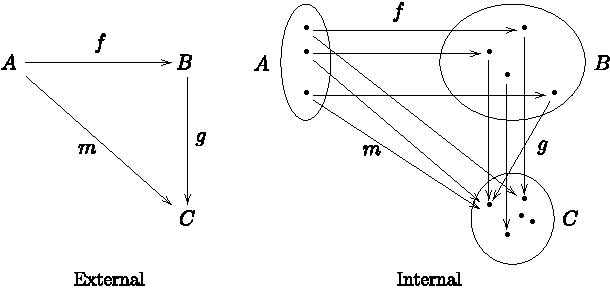
\includegraphics[width=0.8\columnwidth]{fig/intextdiag.pdf}
\end{center}
\caption{In the external diagram on the left one simply considers \emph{objects} such as $A$,$B$, and $C$ and morphisms between them $f$, $g$, and $m$. The internal perspective, which in this case is specific to the category of $\mathbf{Sets}$, demonstrates the particular manner in which the equation $g \circ f = m$ may be satisfied in terms of the internal structure of the objects $A$, $B$, and $C$. Of course, in this case there are many other ways of satisfying the given equation; however, there are also questions that can be answered about the relationship between $A$, $B$, and $C$ given either $g \circ f = m$ or $g \circ f \neq m$ without necessarily knowing the particular manner in which either equation is satisfied by the relationships among the internal structures of the objects involved.}
\label{fig:intextdiag}
\end{figure}
